\section{Implementation}
\label{sec:implementation}
Our VizAPI tool includes two main phases: (1) data extraction and (2)
visualization. The data extraction phase uses static and dynamic
analysis to collect data about client usages of libraries. The
visualization phase transforms the extracted data into d3 format and makes it
available to users.

In this section, we start by describing the design of our VizAPI
tool. Then, in Section~\ref{sec:design-decisions}, we discuss
alternatives that we could have chosen, including their advantages and
drawbacks.  The goal of this paper is to produce an explanation of our
artifact that will be helpful to other researchers, including in
particular an exploration of the design space for tools like ours.

\subsection{VizAPI}
Although it is not the focus of this paper, we briefly describe VizAPI
to enable discussions of its design and implementation.
The VISSOFT paper~\cite{venkatanarayanan22:_vizap}
and the first author's MMath thesis~\cite{venkatanarayanan22:_study_lever_api_usage_patter} explain VizAPI in more detail.

We first define the terms ``client'', ``library'' and ``dependency'', which we use throughout this paper. A ``client'' is a software component which directly uses some functionality of an external component, which is the ``library''. Any external component that the ``library'' directly uses is a ``dependency'' of that library; libraries may also have ``transitive dependencies''.

VizAPI visualizes API usages---from clients to libraries, but also from libraries to clients and between libraries (including transitive dependencies). The goal of VizAPI is to provide a heuristic for developers considering the impacts of changes to libraries. VizAPI incorporates information from static and dynamic analyses.  We have made VizAPI publicly available\footnote{\url{https://github.com/SruthiVenkat/api-visualization-tool}}.

\begin{figure}[h]
\begin{center}
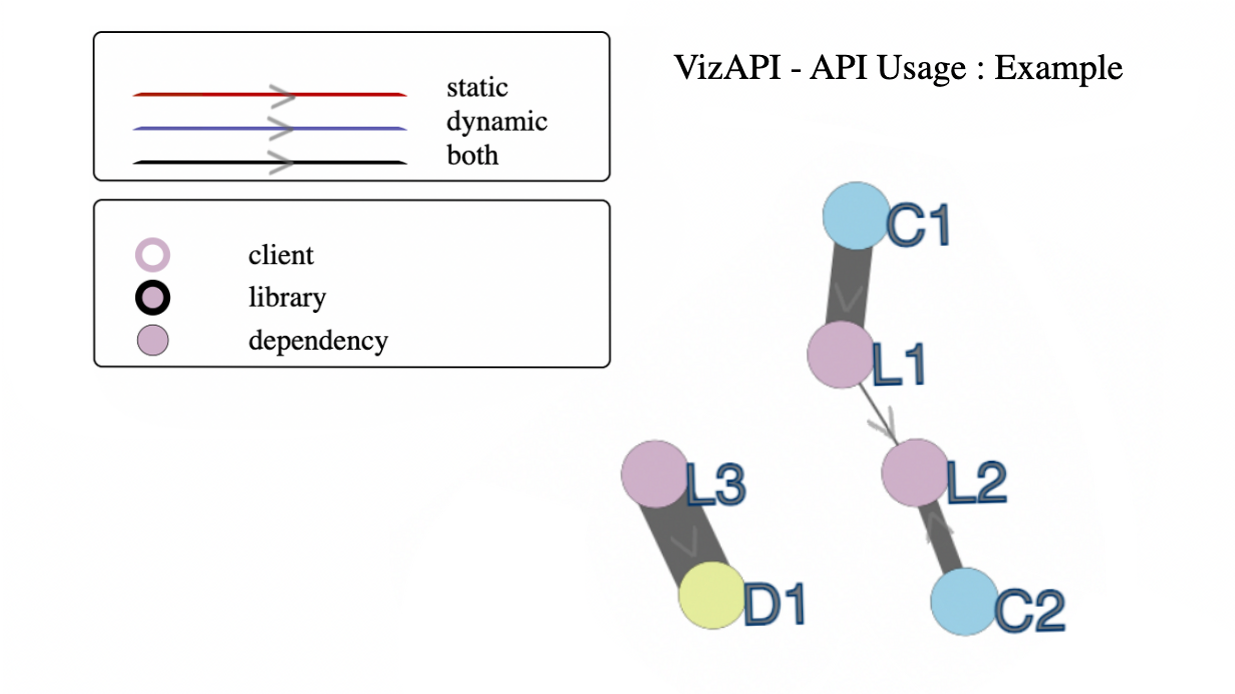
\includegraphics[height=4cm,width=7cm]{images/intro-example.png}
\caption{VizAPI visualization of client C which calls library L, itself dependent on dependency D.}
\label{fig:example}
\end{center}
\end{figure}

Figure~\ref{fig:example} illustrates a VizAPI usage scenario, from the perspective of a client developer worried about breaking changes from the library. It shows plain Java client $C$ (blue nodes) and library $L$ (purple nodes). Library $L$ has packages $L_1$, $L_2$, and $L_3$. $C$ calls into $L_1$ and $L_2$. Internally, within $L$, $L_1$ and $L_2$ call into each other, but not into $L_3$. The VizAPI result, with no edges from $C$ directly to $L_3$, allows a developer to conclude that breaking changes in $L_3$ will not affect $C$. Also, if only $L_3$ uses an external dependency $D$ (yellow node), then $C$ will not need $D$ to be on its classpath.

To do this, VizAPI needs to collect information about dependencies. We provide a few examples of dependencies---enough to give the idea of what VizAPI is looking for, but not an exhaustive list.

\paragraph{Vanilla invocations} The goal here is to capture information about method calls between components. This information can be approximated statically using Class Hierarchy Analysis, as we describe below. Furthermore, it can also be captured precisely at runtime, at least for the invocations that happen on a particular set of executions.

\paragraph{Dynamic proxies and reflective calls} We use a dynamic approach for recording these calls to avoid needing to make hopelessly conservative approximations.

\paragraph{Service Loaders} This Java API allows Java programs to dynamically load additional code, typically plugins. The plugins would declare a published interface, which we can record statically. We are interested in uses of the published interface as well as dynamic calls that exceed the public interface.

\subsection{Static Analysis and Instrumentation}
\label{subsec:static}
Our VizAPI tool integrates data from both static and dynamic analysis.
It turns out that a simple (rather superficial) static analysis suffices
for our purposes, and we describe parts of it here. Section~\ref{sec:design-decisions}
discusses when the use of more sophisticated analyses is appropriate, and
how to incorporate such analyses in an analysis pipeline.

For VizAPI, we chose Javassist~\cite{chiba00:_load_struc_reflec_java} to
perform class hierarchy analysis on components and create a static call
graph. We also use Javassist to instrument the code so that we can
collect dynamic analysis data; we discuss that part in
Section~\ref{subsec:dynamic}. Figure~\ref{fig:workflow} summarizes our
(static) data capture and (dynamic) instrumentation workflow.  \\

\begin{figure*}[h]
 \begin{center}
\resizebox{0.9\textwidth}{!}{
  \begin{tikzpicture}
    \node[block] (client) {client};
    \node[block,below=1cm of client] (library) {library};

    \draw (library) -- node[left] (depends) {depends on} (client);

    \node[above left=.75em of client] (ja) {\begin{minipage}{7em} modify \\with Javassist \end{minipage}};
    \draw[-Latex] (ja) -> (client);
    \draw[-Latex] (ja) to [->,bend right=35] (library.west);

    \node[block, above right=2em of client,xshift=-2em] (olib) {other library};
    \draw (client) -- node[right,xshift=.1em] (also) {also depends on} (olib);

    \node[oval,right=of depends] (test) {maven: run tests};

    \draw[-Latex] (client) to [->,bend left=15] (test);

    \node[block, right=10em of client] (output) {test output};
    \node[block, right=10em of library] (raw) {raw API usage info};

    \draw[-Latex] (test) to (output);
    \draw[-Latex] (test) to (raw);

    \node[oval, right=of raw] (Py) {Python scripts};
    \draw[-Latex] (raw) to (Py);

    \node[block, right=1em of Py] (viz) {D3 visualizations};
    \draw[-Latex] (Py) to (viz);
  \end{tikzpicture}
}
  \caption{Our instrumentation workflow. Using Javassist, we analyze and instrument clients and run their test suites. (We process the generated data with Python scripts to create D3 visualizations for VizAPI.)}
  \label{fig:workflow}
 \end{center}
\end{figure*}

\paragraph{Vanilla invocations}
The standard case is simple. At every invoke instruction in every
loaded method which transfers control between the client and the
library, we record a static dependency (using a Class Hierarchy
Analysis callgraph that we compute) and add code to dynamically record
the invoke by incrementing a counter just before the invoke
executes. Note that we handle all Java invocation types, including
virtual and even dynamic invokes. Crossing the client/library boundary
includes conventional calls from the client to the library as well as
callbacks from the library to the client.  Because we instrument
libraries, we can record both invocation directions.

Since Class Hierarchy Analysis is so straightforward, we implemented
it ourselves: when we first read the class files, we record
inheritance relationships between classes; then, when we re-visit all
methods, we add an edge between the caller and its potential callees
(as earlier recorded).  In any case, we need the inheritance
relationships: when a client extends a library class, that constitutes
a different kind of dependency, which we also record.

\paragraph{Service Loaders} We are particularly interested in bypasses of 
services that use the \texttt{ServiceLoader} API. Before the instrumentation, we record a list 
of services and their implementations by statically inspecting files in \texttt{src/main/resources/META-INF/services}. This gives a static list of dependencies; anything beyond this list that we observe dynamically would be a service bypass.

\subsection{Dynamic Analysis}
\label{subsec:dynamic}
We collect data about client usages of libraries by running client
test suites under instrumentation. The instrumentation records API
uses which cross client/library boundaries, closely mirroring the API
usage patterns
in~\cite{venkatanarayanan22:_study_lever_api_usage_patter}.. We first
describe how we capture specific dependencies between components, and
then discuss our instumentation implementation.

\paragraph{Vanilla invocations} The code that we inserted during the
static analysis/instrumentation phase keeps track of invocation counters
and writes them out upon program termination.

\paragraph{Dynamic proxies and reflective calls}
We specially handle invocations of
\texttt{java.lang.reflect.Method.invoke()}, a distinguished method
used to invoke dynamic proxies and reflective calls, dynamically
recording details of the calls that we intercept. It is possible for
static analyses to resolve a subset of such calls using clever
techniques. Our machinery does not provide enough information to
statically resolve this dependency, but we have full visibility into
such calls dynamically.

\paragraph{Service Loaders} In the dynamic phase, we use the statically recorded information to dynamically detect service bypasses which are direct uses of service implementation 
classes in clients, either through instantiations, casts or reflection. To do so, we intercept calls 
to method \texttt{load()} in classes with name \texttt{Service*Loader} and record any calls to methods beyond 
the published interface that we have recorded statically.

\paragraph{Instrumentation implementation}
We identify interactions across the client/library boundaries by
inspecting JAR files of each software component (clients and
libraries) to obtain a list of classes for every component. We
associate classes and their members to components based on these
lists. 

\todo{where agent}

We first recompile and instrument the classes. Using Maven, we build JAR
files that contain source code only. This ensures that we do not
capture library uses meant solely for unit testing.  We recompile
these source code classes, and then we instrument them using Javassist
APIs that modify the bytecode. We examine each class and its members,
and insert instrumention that increments counters every time there is
an interaction with a different JAR. The instrumentation also builds
dynamic call graphs.

In the dynamic analysis phase, we modify the build system of each
client (Maven) to run its provided tests on instrumented code,
obtaining dynamic call graphs.  The static analysis captures the
following patterns: vanilla invocations, field accesses, class usages,
setAccessible(), annotations and inheritance information. The dynamic
analysis captures all dynamic uses of those patterns and additionally
reflection, dynamic proxies and service loader bypasses.

Because we executed each of the clients' test suites to collect data about how the clients use all of their dependencies, our data therefore includes not just interactions between our clients and the 11 libraries sampled, but also ``bycatch''---that is, other libraries that are also called by the clients (``also depends on'' in Figure~\ref{fig:workflow}) and the libraries. The total static transitive closure of dependencies of our clients includes 4297 components. Section~\ref{sec:benchmark} discuss our benchmark suite in more detail.

While our current benchmark set consists of 101 projects, it is possible to run both our static and dynamic analysis tool and the VizAPI visualization tool on new libraries and clients. However, when either tool is run by a library developer, they are required to provide a specific set of clients that they wish to observe as input to the tools. Libraries.io can be used to find popular clients of libraries---it provides a dependency tree based on projects' packaging information.


\subsection{Visualization System}
\label{subsec:vis-system}

\begin{figure*}[h]
\begin{center}

\subfloat[Usage Scenario 1: Library \textit{jsoup} (pink with dark borders), called by two clients, \textit{ez-vcard} (hollow with purple border) and \textit{JsoupXpath} (hollow with pink border). Exploration shows that internal jsoup packages aren't called directly by clients.
\label{fig:usagescenario1}]
{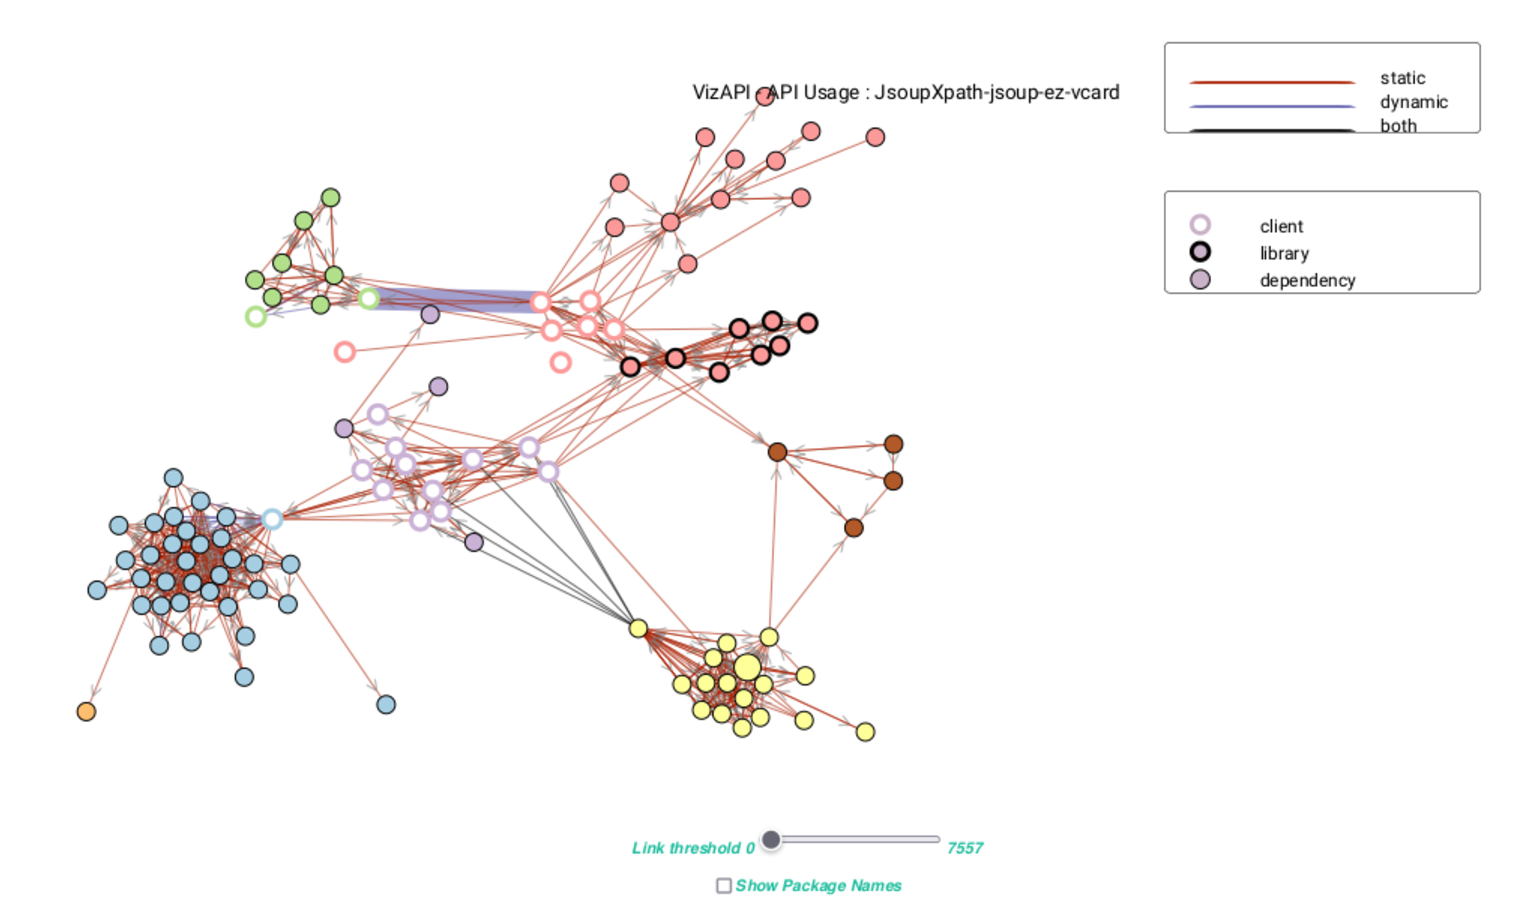
\includegraphics[width=16cm]{images/usage-scenario1.pdf}}
\hspace{7mm}

\subfloat[Usage Scenario 2: Client \textit{dataprocessor} (hollow, orange border) calls only one package in library \textit{fastjson} (green fill).
\label{fig:usagescenario2}]
{
\makebox[16cm]{
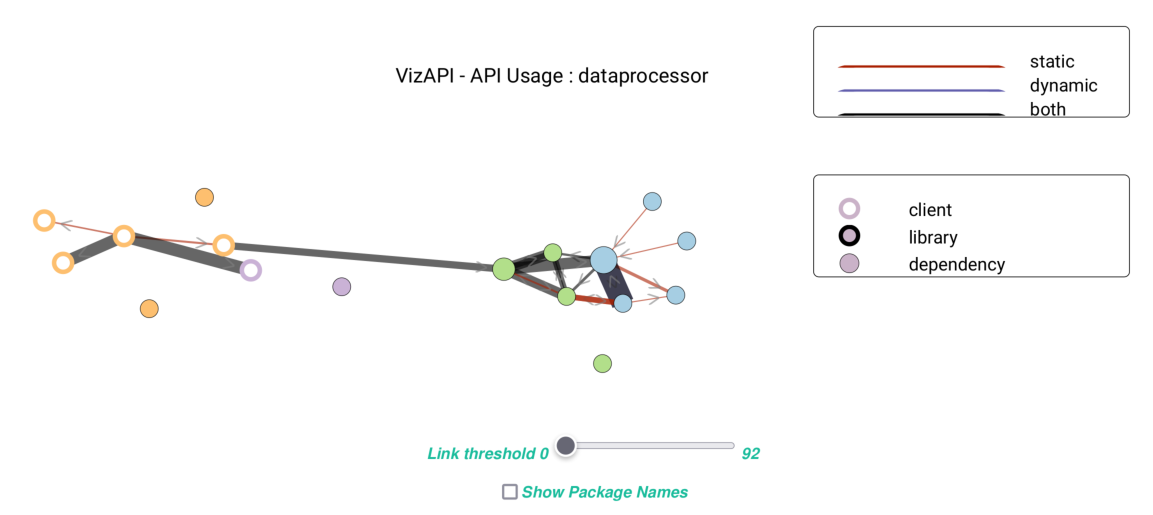
\includegraphics[width=11cm]{images/usage-scenario2.pdf}
}
}
\caption{\label{fig:usagescenarios} VizAPI Usage Scenarios.}

\end{center}
\end{figure*}


Once we have generated static and dynamic analysis data using our tool, we use a modified version
of the d3graph\footnote{\url{https://pypi.org/project/d3graph/}} library in Python to generate a d3js\footnote{\url{https://d3js.org/}}
visualization. The modifications that we made to the d3graph  library in Python in Python include multiple styling changes (for example, changing node styles based on whether it is a client, library or dependency),
legends, and a toggle to show all package names. 
The graphs in Figures~\ref{fig:example}, \ref{fig:usagescenario1}, and \ref{fig:usagescenario2} are examples of graphs produced by VizAPI.

VizAPI graphs are force-directed graphs based on the frequency of
interactions between different software components.  Each node is a
set of one or more packages that belong to the same JAR.  There are
three categories of nodes: clients are represented by nodes with white
interiors; libraries by nodes with filled interiors and black borders;
and dependencies (called by libraries but not clients) by nodes with
filled interiors and normal borders.  We coalesce nodes if they
originate from the same JAR and have the same incoming and
outgoing edges.

Each edge is directed
from the source package(s) to the target package(s) and represents an interaction 
(invocations, fields, annotations, subtyping) between packages. 
The thickness of each edge reflects the frequency of interactions between the source and the target.
Double-clicking on a node emphasizes its direct interactions with other packages while fading out the rest of the graph.

We run a Python implementation of the Louvain clustering algorithm~\cite{blondel2008fast}, and make the clusters 
visible by colouring nodes based on cluster.
This means that the same colour could indicate nodes (of the same category) from the same or different JARs.
Hovering on a node shows the list of packages and 
the JAR that they belong to, 
formatted as “jar : $\langle$space separated list of packages$\rangle$”. 
